\documentclass{article}
\usepackage{latexsym}
\usepackage{amsmath}
\usepackage[a4paper]{geometry}
\usepackage{fullpage}
\usepackage{hyperref}
\usepackage{booktabs}
\usepackage{graphicx}
\usepackage{tikz}
\usepackage{xcolor}
\usepackage[export]{adjustbox}
\usepackage{comment}
\usepackage{subcaption}
\usepackage[style=iso]{datetime2}
\usepackage{cleveref}
%\usetikzlibrary{calc}
\usetikzlibrary{arrows,positioning} 
\tikzset{
    %Define style for course boxes
    courseboxv/.style={
           rectangle,
           draw=blue!50!black, very thick,
           fill=blue!10,
           minimum height=8cm,
           minimum width=4cm,
           text width=3.9cm,
           text centered,
           font=\bfseries\sffamily},
    courseboxh/.style={
           courseboxv,
           minimum height=4cm,
           minimum width=8cm,
           text width=7.9cm},
    courseboxhh/.style={
           courseboxh,
           minimum height=4cm,
           minimum width=16cm,
           text width=15.9cm}
}
\def\frameseparation{1.5cm}
\def\scalingfactor{.8}

\newcommand{\secref}[1]{Section~\ref{sec:#1}}
\newcommand{\secreff}[2]{Sections \ref{sec:#1} and \ref{sec:#2}}
\newcommand{\eqnref}[1]{Equation~\eqref{eq:#1}}
\newcommand{\eqnreff}[2]{Equations \eqref{eq:#1} and \eqref{eq:#2}}
\newcommand{\eqnrefff}[3]{Equations \eqref{eq:#1}, \eqref{eq:#2} and \eqref{eq:#3}}
\newcommand{\figref}[1]{Figure \ref{fig:#1}} 
\newcommand{\figreff}[2]{Figures \ref{fig:#1} and \ref{fig:#2}}
\newcommand{\figrefff}[3]{Figures \ref{fig:#1}, \ref{fig:#2} and \ref{fig:#3}}
\newcommand{\tabref}[1]{Table~\ref{tab:#1}}
\newcommand{\tabreff}[2]{Tables~\ref{tab:#1} and \ref{tab:#2}}
\newcommand{\tabrefff}[3]{Tables~\ref{tab:#1}, \ref{tab:#2} and \ref{tab:#3}}

\def\year{2024--2025}
\title{EITA65 Design of Systems for Digital Transformation\\\year}
%\title{EITA65 Digitalisering -- realisering och systemdesign med användarperspektiv\\\year}
\author{\huge Microservices\\Drone Project -- Part 2}
%\\Version \DTMnow}
%\date{}

\begin{document}
\newgeometry{left=2.5cm,right=2.5cm,bottom=1.5cm}% for placing course schematic lower on first page
\clearpage\maketitle
\thispagestyle{empty}% to remove page numbering on first page

\begin{itemize}
\item 
\includegraphics[width=3mm]{person.png}
\includegraphics[width=3mm]{person.png} This project will be done in pairs, but you will work \textit{together} in groups of 3 or 4.
\item You will not get detailed step-by-step instructions. Figuring out how to reach the goal is part of the project. (being a collaborative doer)
\item The results of this project part will be used in the next, so document your work.
\end{itemize}

\vspace{.1cm}
\begin{center}
\begin{tabular}{l}
\toprule[1.5pt]
\parbox{0.8\linewidth}{
\vspace{.2cm}{\Large Learning goals:}
\begin{itemize}
\item Becoming familiar with web server development and microservices
  \begin{itemize}
  \item Understanding interactions with multiple servers.
  \item Learn to interact with a Redis database. 
  \end{itemize}
\item Practicing collaboration skills.
\end{itemize}}\\
\bottomrule[1.5pt]
\end{tabular}
\end{center}
\vfill
\begin{center}
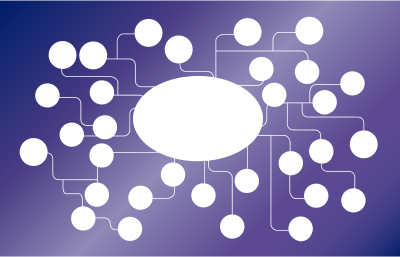
\includegraphics[width=100mm]{networkclipart.png}
\end{center}
\vspace{2cm}

\begin{comment}
\begin{center}
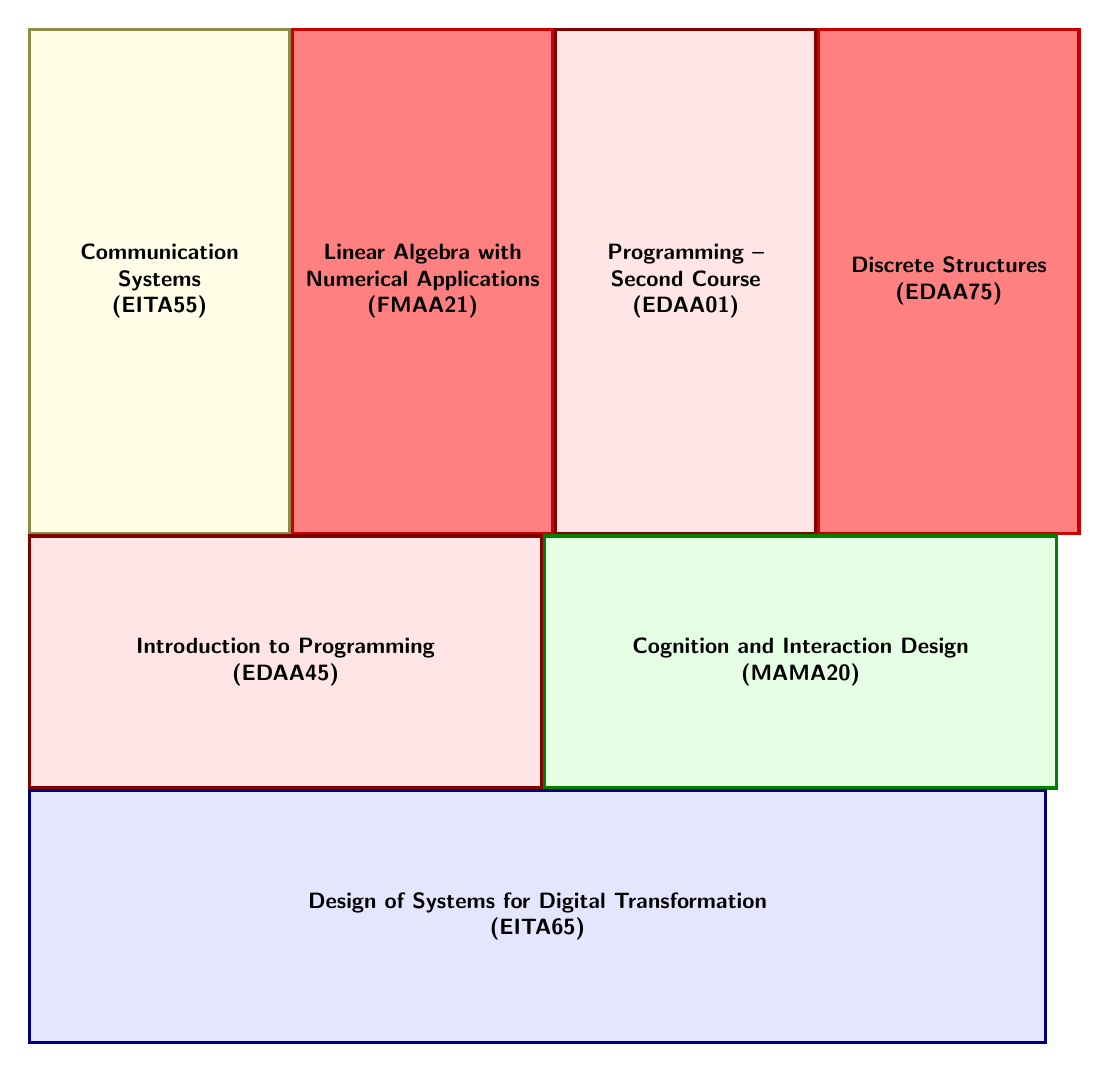
\begin{tikzpicture}[>=latex, node distance=0cm,scale=\scalingfactor,every node/.style={scale=\scalingfactor}]
\node[courseboxv, draw=yellow!50!black, fill=yellow!10] (EITA55) {Communication Systems\\(EITA55)};
\node[courseboxv, draw=red!80!black, fill=red!50, anchor=west] (FMAA21) at (EITA55.east){Linear Algebra with Numerical Applications\\(FMAA21)};
\node[courseboxv, draw=red!50!black, fill=red!10, anchor=west] (EDAA01) at (FMAA21.east){Programming -- Second Course\\(EDAA01)};
\node[courseboxv, draw=red!80!black, fill=red!50, anchor=west] (EDAA75) at (EDAA01.east){Discrete Structures\\(EDAA75)};
%\node[courseboxh, preaction={clip, postaction={fill=red!10, draw=red!50!black, line width=2mm}}, anchor=north west] (EDAA45) at (EITA55.south west){Introduction to Programming\\(EDAA45)};
\node[courseboxh, draw=red!50!black, fill=red!10, anchor=north west] (EDAA45) at (EITA55.south west){Introduction to Programming\\(EDAA45)};
%\node[courseboxh, draw=green!50!black, fill=green!10, anchor=west] (MAMA20) at (EDAA45.east){Cognition and Interaction Design\\(MAMA20)};
\node[courseboxh, draw=green!50!black, fill=green!10, right=of EDAA45] (MAMA20) {Cognition and Interaction Design\\(MAMA20)};
\node[courseboxhh, anchor=north west] (EITA65) at (EDAA45.south west){Design of Systems for Digital Transformation\\(EITA65)};
%\node[anchor=south east, inner sep=2pt, font=\bfseries\sffamily\scriptsize] at (EDA625.south east) {Helsingborg};
%\path[->,draw=black,dotted,thick] (EIT060.east) -- (EITF05.west);
%\path[->,draw=black,dotted,thick] (EIT060.south) -- (EITN50.north);
%\path[->,draw=black,dotted,thick] (EITF05.south) -- (EITN41.north);
%\draw[draw=blue!50!black, very thick] ($(EIT060.north west)+(-\frameseparation,\frameseparation)$) rectangle ($(EDA625.south east)+(\frameseparation,-\frameseparation)$);
\end{tikzpicture}
\end{center}
\end{comment}

\restoregeometry
\newpage


\section{Introduction}
In this project part you will get more acquainted with a Flask web server and a Redis server. You will also learn how to build an application with multiple web servers. You will start to get an idea about microservices, and how to implement a microservice architecture for a big system.

We still work with the Drone simulation system in this part, which is more or less the same as the one we looked at in Part 1, Drone simulation on Raspberry Pi, but we will add a Redis database to the system, and store longitude and latitude data in the database.
You will use the code from  {\color{blue}\href{https://github.com/rogerhenriksson/InfoCom-Drone-2-Microservices}{GitHub repository} }in this instruction. As for Part 1, you are recommended to fork and clone from your own repository. Before you run the code, read the instruction and fill in with your own code in the places pointed out by comments. Otherwise you may get error messages.

You can replace the \verb!get_direction()! function in \verb!pi_controller.py! with the one you created in Part 1 if you want, but keep \verb!SERVER_URL! the same as the file provided for this instruction. 


\noindent{\bf Note: }\parbox[t]{14cm}{{You will get some questions marked in red in this instruction. You need to write down the answers and show to the TAs after you finish the lab.}}\vspace{0.2cm}

\section{Application Architecture}

In this part, we will use two Flask servers for different jobs. This type of implementation is very common for today's web applications. Look up \textit{microservice architecture} to get to know something more about it. A feature of this architecture is that each service is only responsible for a small job of a large application, but they are interconnected in some way and communicate underneath.

A very typical example of this type of application is the microservice demo developed by Google \cite{MD}, it is an online boutique with all functionalities a web shop should have, and the architecture of this application is shown in \Cref{fig:hipster}. As a client of this application, you only get access to the frontend to browse the shop, but you do not directly see how the other components are connected and interact to provide you other services that are displayed on the fronted website.

\begin{figure}[h!]
    \centering
    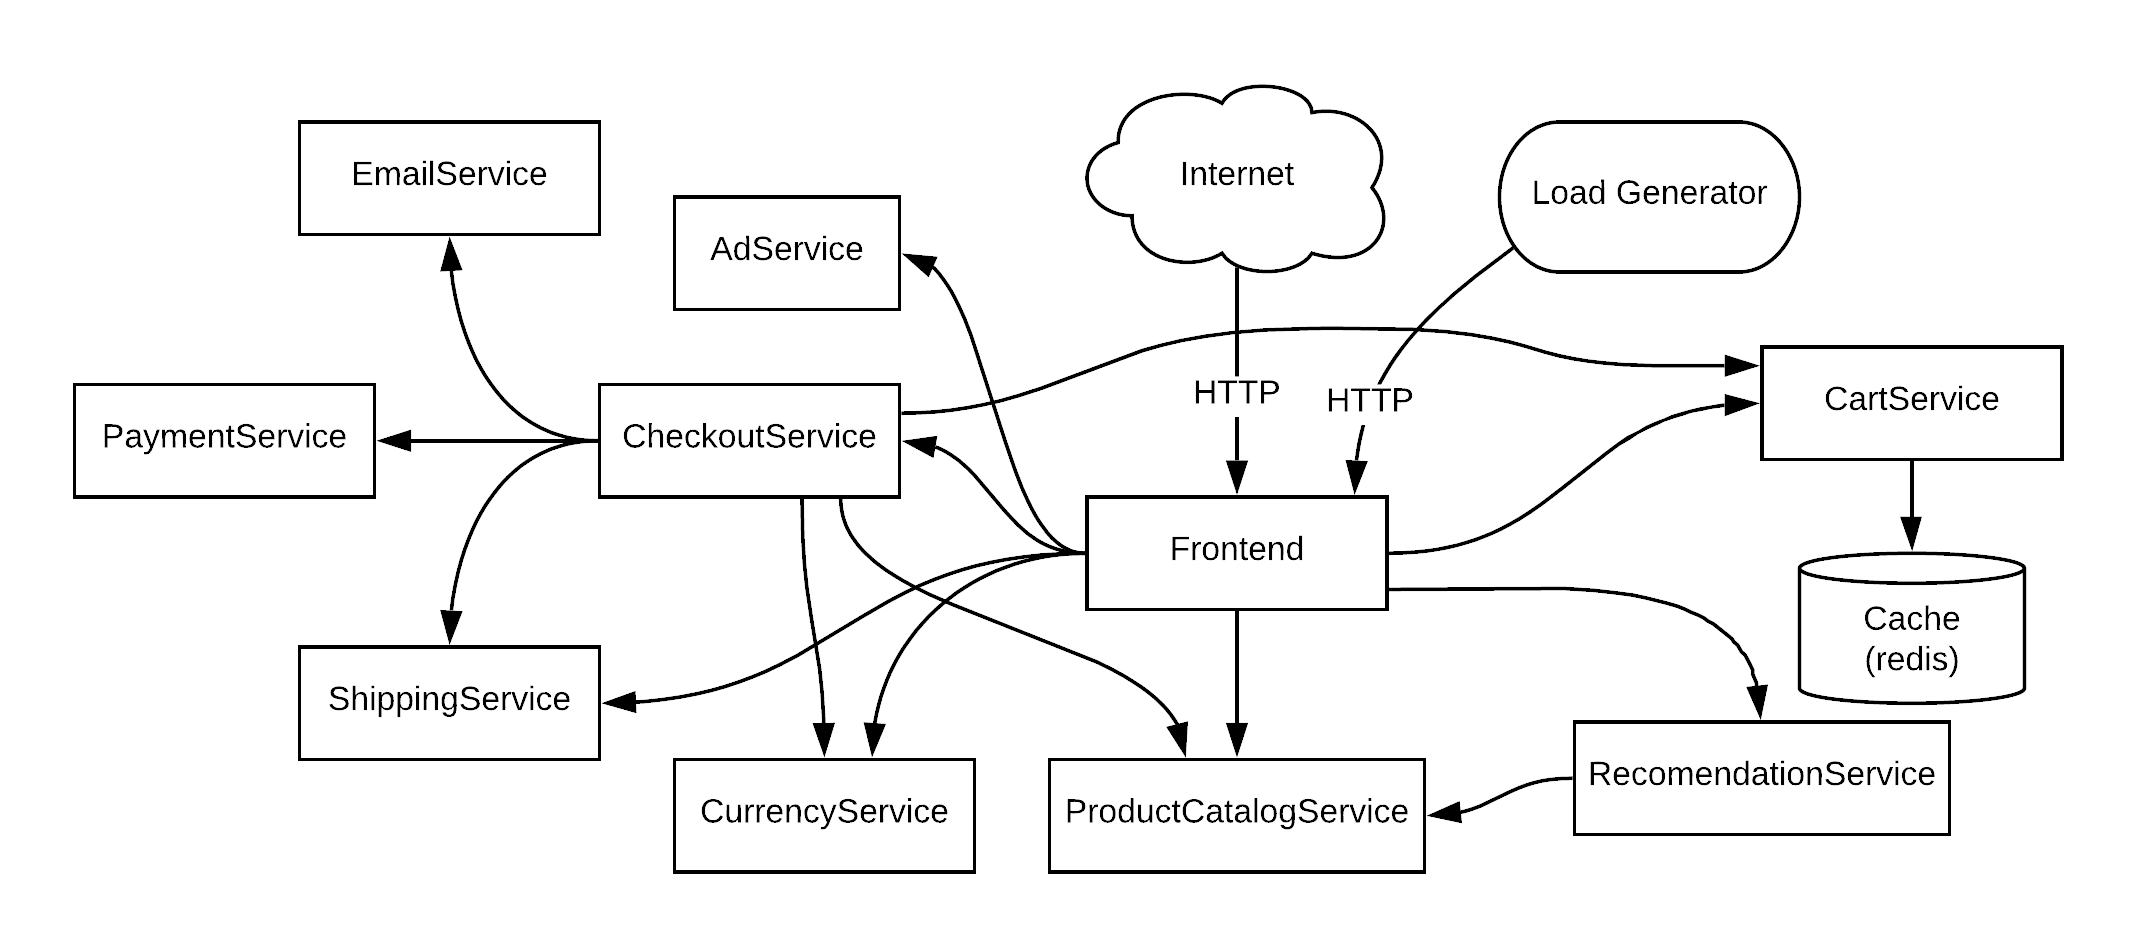
\includegraphics[width=150mm]{architecture-diagram.png}
    \caption{Google's microservice demo architecture.}
    \label{fig:hipster}
\end{figure}

For our drone simulation application, the architecture is much simpler than Google's online boutique. You can see our architecture schematic in \Cref{fig:drone} (arrows indicate direction of requests). As you may remember, in the previous Cloud Services assignment, you had your Raspberry Pi send data directly to the Redis database on your VM in the cloud. In order to do that, you need to run your Redis server under \verb!unprotected-mode! on the VM. It is unsafe and not recommended in any kind of application development. So in this lab, when we introduce a Redis database to the system, we also add a database frontend, so that the database is hidden behind the frontend, and the client is not allowed to write data to the database directly. Instead, the database frontend will act as a data broker, receiving, filtering and passing along the \textit{accepted} data. In short, the data broker (the database frontend) is put in place to protect the database so that we can have some degree of control over who puts what data where in the database.

\begin{figure}[h!]
    \centering
    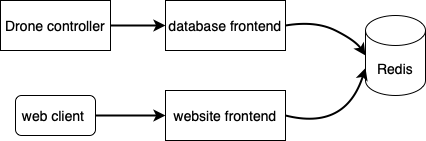
\includegraphics[width=80mm]{drone-system-architecture.drawio.png}
    \caption{Application architecture of a drone simulation system.}
    \label{fig:drone}
\end{figure}

\noindent{\bf Question 1: }\parbox[t]{13cm}{\textcolor{red}{Now go through the provided code, and find out which script matches each component, and what is the web client in this system.}}\vspace{0.5cm}

\noindent{\bf Question 2: }\parbox[t]{13cm}{\textcolor{red}{As mentioned above, we use two Flask servers in the system, write down the URL of each web server.}}\vspace{0.5cm}

\noindent{\bf Question 3: }\parbox[t]{13cm}{\textcolor{red}{Write down what requests are made and what data are sent over each arrow in \Cref{fig:drone}. Note that, the arrow directions don't mean date write/read, but only the directions to make write/read request.}}\vspace{0.5cm}

\section{Write your own}

Some parts in the provided code are omitted. You need to fill in the code for the functions pointed out, and complete the functionality required, as indicated by underlying comments. When you have completed all the code, you should be able to run the application by following the instructions in \verb!README.md! and get no error. The functionalities you should have with each server are:
\begin{itemize}
    \item The database frontend should receive the HTTP request from the drone controller. The request contains data about the drone movement along longitude and latitude. The server needs to update the drone's OSM coordinates with movement values and refresh the data in the database.
    \item The website frontend should keep reading the most recently recorded longitude and latitude data from the database, and display the location on the SVG map.
\end{itemize}

Before you start your web servers, remember to first check that the Redis server is running. If not, start it! If you are using your own computer or you reinstalled the operating system of your Raspberry Pi, you need to install Redis first. When you have all your web servers and the database running, you can control the drone on the website with your keyboard or the joystick, exactly the same way you did in the previous assignment, Drone simulation on Raspberry Pi. But the underlying system architecture has now changed. {\textcolor{red}{You need to show the TAs your completed task when you have completed all your code}}.
%\newpage
%\section{Hint for MAC OS}
%\label{sec:mac}
%If you run the web server on MAC OS, you may, depending on your OS version, get problems with \verb!pip3!. MAC has Python3 installed by default in the system, but not \verb!pip3!. There are several ways to install \verb!pip3! if you use the search phrase \textit{How to install pip3 on MAC OS}. The easiest one you find may be \verb!brew install python3!. The command \verb!brew! is the most popular package manager on MAC OS (like \verb!apt! in Debian), but when you install with \verb!brew!, you install the whole python3 again in your system, but in a different path. This path is not in your default system PATH, so your computer will not understand that you wants to use the newly installed python3. Therefore, you need to add the new path to your system PATH in \verb!~/.bash\_profile! or \verb!~/.zshrc!, then \verb!source! the changed file and you should be able to use the newly installed \verb!python3! and \verb!pip3!.

% {\bf Hint 1: }\parbox[t]{14cm}{Check for updates to this document. Instructions may have been clarified in a more recent version. You can find the version number of the document on the very first page. The version number is the compile-date of the document in ISO-format~\cite{iso-date-time}.}\\
% {\bf Hint 2: }\parbox[t]{14cm}{To avoid rewriting many commands, you can use the keys \texttt{arrow up} and \texttt{arrow down} to go back and forth between the commands that you just wrote.}\\
% {\bf Hint 3: }\parbox[t]{14cm}{To paste commands into the terminal you can use \texttt{Ctrl + Shift + V}}\\
% {\bf Hint 4: }\parbox[t]{14cm}{tab in instructions}\\
% {\bf Hint 5: }\parbox[t]{14cm}{To avoid rewriting many commands, it can be a good idea to write all steps in a batch-file or shell script. Then you can also reuse the batch file for the second project.}
\vspace{1cm}
\begin{center}
\huge Good luck!
\end{center}

\begin{thebibliography}{10}
\bibliographystyle{plain}

\bibitem{MD} Google's microservice demo, \url{https://github.com/GoogleCloudPlatform/microservices-demo}, last accessed on 2025-01-07.

% \bibitem{OSM} OpenStreetMap, \url{https://www.openstreetmap.org/#map=14/55.7059/13.2005}, last accessed on 2021-11-08.

% \bibitem{deco} Python decorator, \url{https://python-3-patterns-idioms-test.readthedocs.io/en/latest/PythonDecorators.html}, last accessed on 2021-11-08.


\end{thebibliography}

\end{document}
